\chapter{Stationäre Ströme}

\section{Grundgleichungen und Vektorpotential}

Wenn wir stationäre Ströme betrachten, dann gilt ebenso wie in der Elektrostatik, dass die Felder zeitunabhängig sind: $\dot{\vec{E}} = 0, \dot{\vec{B}}=0$. Außerdem ist div $\vec{j} = 0$.\
Da für das $\vec{B}$-Feld unter diesen Bedingungen gilt, dass rot $\vec{B} = \mu_0 \ \vec{j}$, ist es nicht möglich ein $\psi$ zu finden, sodass grad $\psi = \vec{B}$. Anstattdessen macht man sich die Quellenfreiheit eines Wirbelfelds zu nutze und führt ein Vektorpotential $\vec{A}(\vec{r})$ ein, sodass:

\begin{equation*}
\vec{B}(\vec{r}) = \rot \vec{A}(\vec{r})
\end{equation*}

$\vec{B}$ bestimmt $\vec{A}$ bis auf Eichtransformation $\vec{A}\ \rightarrow \ \vec{A} \ + \ \grad \vec{chi}$ eindeutig, da beide Vektorpotentiale das selbe $\vec{B}$-Feld liefern. Bei spezieller Wahl von $\chi$ spricht man von fixierter Eichung.\
Mit der Einführung von $\vec{A}$ folgt mit $\frac{1}{\mu_0}\ \rot \vec{B} = \vec{j}$:

\begin{equation*}
\frac{1}{\mu_0}\ (\rot\rot\vec{A})=\vec{j} \quad \text{bzw.} \quad \grad\div \vec{A}\ - \ \laplace\vec{A}=\mu_0 \ \vec{j}
\end{equation*}

Es bietet sich an, die Eichung div $\vec{A} = 0$ (\textsc{Coulomb}-Eichung) zu wählen, sodass folgt:

\begin{equation*}
-\laplace\vec{A}=\mu_0 \ \vec{j}
\end{equation*}

Eine ähnliche Gleichung haben wir mit der \textsc{Poisson}-Gleichung $-\epsilon_0 \ \laplace\varphi = \rho$ in der Elektrostatik hergeleitet und diese mit $\varphi = \frac{1}{4\pi\epsilon_0}\Int{}{}{V'}\frac{\rho(\vec{r})}{|\vec{r}-\vec{r}'|}$ gelöst.\ \\
Analog erhalten wir auch die Lösung für $\vec{A}$:

\begin{align*}
\vec{A}(\vec{r}) = \frac{\mu_0}{4\pi}\Int{}{}{V'} \ \frac{\vec{j}(\vec{r})}{|\vec{r}-\vec{r}'|} \qquad \text{mit div }\vec{A} = 0 \\
\ \\
\vec{B}(\vec{r}) = \rot \vec{A}(\vec{r}) = \frac{\mu_0}{4\pi}\ \Int {}{}{V'} \ \frac{\vec{j}(\vec{r})\times (\vec{r}-\vec{r}')}{|\vec{r}-\vec{r}'|^3}
\end{align*}

Die Kontrolle, ob div $\vec{A} =0$ ist, ergibt:

\begin{equation*}
\div\vec{A}(\vec{r}) = \frac{\mu_0}{4\pi} \ \Int{}{}{V''}\ \frac{1}{r''} \ \underbrace{\div\vec{j(\vec{r}+\vec{r}''})}_{=0}=0 \qquad \text{mit } \vec{r}'' = \vec{r}'-\vec{r}
\end{equation*}

\section{Leiterschleifen}

\begin{wrapfigure}[]{l}[0cm]{0cm}
	\raisebox{0pt}[\dimexpr\height-1\baselineskip\relax]{
		\colorbox{hgrey}{
			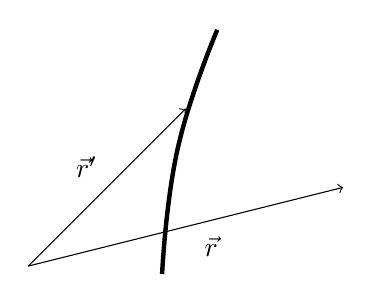
\begin{tikzpicture}
			
			\draw[ultra thick] plot[smooth, tension=.8] coordinates {(1.7,-0.1) (1.9,1.5) (2.4,3) };	
			\draw[->] (0,0) -- node[above left]{$\vec{r}'$} (2,2);
			\draw[->] (0,0) -- node[below right]{$\ \vec{r}$} (4,1) ;
			
			
			\end{tikzpicture}
		}
	}
	\caption{Ausschnitt einer Leiterschleife}
\end{wrapfigure}
Wir betrachten einen Leiter der Dicke $d$ an der Position $\vec{r}'$. Für "dünne" Leiter, d.h. $d \ll |\vec{r}-\vec{r}'|$, kann man d$V' \vec{j}(\vec{r})$ vereinfachen zu: d$\vec{r}' \cdot I$, wobei das Längenelement d$\vec{r}'$ entlang des Leiters verlaufen soll.\
Für mehrere Leiter $\mathcal{L}_n$ folgt demnach für das Vektorpotential:

\begin{align*}
\vec{A}(\vec{r}) &= \frac{\mu_0}{4\pi}\ \sum_n \ I_n \ \int\limits_{\mathcal{L}_n} \frac{\mathrm{d}\vec{r}'}{|\vec{r}-\vec{r}'|}\\
\ \\
\overset{\vec{B}= \rot\vec{A}}{\Rightarrow} \quad \vec{B}(\vec{r}) &= \frac{\mu_0}{4\pi} \ \sum_n \ I_n \int\limits_{\mathcal{L}_n} \frac{\mathrm{d}\vec{r}' \times (\vec{r}-\vec{r}')}{|\vec{r}-\vec{r}'|^3}
\end{align*}
\ \\
Diese Gleichung zur Bestimmung des $\vec{B}$-Feldes einer beliebigen Anordnung dünner Leiter nennt man das \textsc{Biot-Savart}-Gesetz.\
\\
\ \\
Betrachten wir nun bei mehreren geschlossenen Leiterschleifen den magnetischen Fluss auf deren Oberflächen $\mathcal{S}_m$:

\begin{equation*}
\Phi = \Iint{\mathcal{S}_m}{}{\vec{A}_{\mathcal{S}_m}}\cdot\vec{B} = \Oint{\partial\mathcal{S}_m}{}{\vec{r}}\cdot\vec{A}
\end{equation*}

Mit \textsc{Biot-Savart} ergibt sich:

\begin{equation*}
\Phi = \frac{\mu_0}{4\pi}\ \sum_n \ I_n \ \Oint{\partial\mathcal{S}_m}{}{\vec{r}}\ \cdot \ \Oint{\partial\mathcal{S}_n}{}{\vec{r}'}\frac{1}{|\vec{r}-\vec{r}'|} \ =: \ \sum_n \ L_{mn} \ I_n
\end{equation*}

\begin{equation*}
\text{mit } L_{mn} = \frac{\mu_0}{4\pi} \ \Oint{\partial\mathcal{S}_m}{}{\vec{r}}\ \Oint{\partial\mathcal{S}_n}{}{\vec{r}'}\frac{1}{|\vec{r}-\vec{r}'|}
\end{equation*}

Die $L_{mn}$ sind die sogenannten \textbf{Induktionskoeffizienten}, welche ebenso wie die Kapazitätskoeefizienten symmetrisch sind: $L_{mn} = L_{nm}$. Für $m=n$ redet man von \textbf{Selbstinduktivitäten} der Leiter, welche allerdings  nicht mit der obigen Formel berechnet werden können, da dann die Näherung der "dünnen" Leiter zusammenbricht.

\section{Magnetischer Dipol}

Für eine geschlossene Leiterschleife der Fläche $\vec{A}_F$, durch die der Ringstrom $I$ fließt, definieren wir das \textbf{magnetische Dipolmoment} $\vec{m}$ wie folgt:

\begin{equation*}
\vec{m} \ := \ I \ \cdot \ \vec{A}_F
\end{equation*}
\begin{equation*}
\text{Dipollimit: } \quad |\vec{A}_F| \ \rightarrow \ 0, \ I \ \rightarrow \ \infty \ \Rightarrow \ |\vec{m}| \ = \ \text{const.}
\end{equation*}

Um das Vektorpotential

\begin{equation*}
\vec{A}(\vec{r}) = \frac{\mu_0 I}{4\pi}\oint\frac{\mathrm{d}\vec{r}'}{|\vec{r}-\vec{r}'|}
\end{equation*}

für diesen Dipol zu berechnen entwickeln wir dieses unter der Näherung großer Abstände zum Dipol( $r\gg a$, wobei $a$ die größte Ausdehnung des Dipols in eine Raumrichtung ist):

\begin{equation*}
\frac{1}{|\vec{r}-\vec{r}'|} \cong  \frac{1}{|\vec{r}|} + \frac{\vec{r}\cdot\vec{r}'}{|\vec{r}|^3} + \dotsc \quad \Rightarrow \quad \oint\frac{\mathrm{d}\vec{r}'}{|\vec{r}-\vec{r}'|} = \underbrace{\frac{1}{r} \Oint{}{}{\vec{r}'}}_{=0} \ + \ \frac{\vec{r}}{r^2}\Oint{}{}{\vec{r}} \circ\vec{r}' \ + \dotsc
\end{equation*}

Umformen ergibt:

\begin{align*}
\Oint{}{}{\vec{r}'} (\vec{r}'\cdot\vec{a}) &= \frac{1}{2}\Bigg[\Oint{}{}{\vec{r}'}(\vec{r}'\cdot\vec{a}) \ - \oint(\mathrm{d}\vec{r}'\cdot\vec{a})\vec{r}'\Bigg] \ + \ \frac{1}{2} \Bigg[\Oint{}{}{\vec{r}'}(\vec{r}'\cdot\vec{a}) \ + \ \oint(\mathrm{d}\vec{r}'\cdot\vec{a})\vec{r}'\Bigg]\\
&= \underbrace{\frac{1}{2}\oint(\vec{r}'\times\mathrm{d}\vec{r}')}_{\text{Fläche }A_F} \times\vec{a} \ + \ \frac{1}{2} \oint\mathrm{d}\left[\vec{r}'(\vec{r}'\cdot\vec{a})\right]\\ 
\ \\
& \Rightarrow \quad \vec{A}(\vec{r}) = \frac{\mu_0 I }{4\pi} \; \vec{A}_F\times\frac{\vec{r}}{r^3} = \frac{\mu_0}{4\pi} \cdot \frac{\vec{m}\times\vec{r}}{r^3}
\end{align*}
\ \\
(zum Vergleich das Potential eines Elektrischen Dipols: $\varphi(\vec{r}) = \frac{1}{4\pi\epsilon_0} \cdot \frac{\vec{p}\cdot\vec{r}}{r^3}$)
\ \\
\begin{align*}
\vec{B}(\vec{r}) = \rot\vec{A}(\vec{r}) &= - \frac{\mu_0 I}{4\pi} \ \nabla \times \left(A_F\times\nabla\frac{1}{r}\right) \ = \ \frac{\mu_0}{4\pi} \ \cdot \ 3(\vec{m}\cdot\vec{r})\vec{r} \ - \ \vec{m}r^2\\
\ \\
&= \ \underbrace{\vec{A}_F \ \laplace\frac{1}{r}}_{(*)} \quad - \quad \underbrace{(\vec{A}_F
	\cdot\nabla)\ \nabla \ \frac{1}{r}}_{= \ \vec{A}_F (\nabla \circ \nabla) \frac{1}{r}}
\end{align*}

$(*) = 4\pi\delta(\vec{r})$ wird im Fernfeld vernachlässigt
\ \\
\ \\
\underline{Ladung auf Umlaufbahn}:$\qquad$ (Ladung $Q$, Masse $M$)

\begin{equation*}
I = \frac{Q}{\tau} \qquad \text{ mit } \qquad \tau \; \hat{=} \; \text{Umlaufzeit}
\end{equation*}
\begin{equation*}
\vec{A}_F = \frac{1}{2}\oint\vec{r}\times\mathrm{d}\vec{r} = \frac{1}{2}\Int{0}{\tau}{t} \ \left(\vec{r}\times\diff{\vec{r}}{t}\right) =\frac{1}{2}\tau \frac{\vec{L}}{M}
\end{equation*}

Das Magnetische Dipolmoment ist also bei einer Ladung auf einer Umlaufbahn eng mit dessen Drehimpuls $\vec{L}$ verknüpft:

\begin{equation*}
\vec{m}  \ =\ I \ \cdot \ \vec{A}_F \ = \ \frac{1}{2} \ \underbrace{\frac{Q}{M}}_{=: g_B} \ \vec{L}
\end{equation*}

(Zum Vergleich das \textsc{Bohr}'sche Magnetron: $\mu_b = \frac{e\hbar}{2m}$)
\ \\
\ \\
\ \\
\ \\
\underline{Allgemeine Stromverteilung}


\begin{equation*}
\vec{m} \ = \ \frac{1}{2} \ \Int{}{}{V} \; \vec{r}\ \times \ \vec{j}(\vec{r})
\end{equation*}

(Zum Vergleich der elektrische Dipol: $\vec{p} = \Int{}{}{V} \vec{r}\rho(\vec{r})$)